\documentclass[border=15pt, multi, tikz]{standalone}
\usepackage{import}
\subimport{../../layers/}{init}
\usetikzlibrary{positioning}
\usetikzlibrary{3d} %for including external image 

\def\ConvColor{rgb:yellow,5;red,2.5;white,5}
\def\ConvReluColor{rgb:yellow,5;red,5;white,5}
\def\PoolColor{rgb:red,1;black,0.3}
\def\DcnvColor{rgb:blue,5;green,2.5;white,5}
\def\SoftmaxColor{rgb:magenta,5;black,7}
\def\SumColor{rgb:blue,5;green,15}
\def\ellipsis{rgb:blue,0.05;green,0.05;red,0.05}
\def\InverseResidual{rgb:blue,255;green,0.05;red,0.05}

\def\FcColor{rgb:blue,5;red,2.5;white,5}
\def\FcReluColor{rgb:blue,5;red,5;white,4}

\begin{document}
\begin{tikzpicture}
\tikzstyle{connection}=[ultra thick,every node/.style={sloped,allow upside down},draw=\edgecolor,opacity=0.7]
%%%%%%%%%%%%%%%%%%%%%%%%%%%%%%%%%%%%%%%%%%%%%%%%%%%%%%%%%%%%%%%%%%%%%%%%%%%%%%%%%%%%%%%%
%% Draw Layer Blocks
%%%%%%%%%%%%%%%%%%%%%%%%%%%%%%%%%%%%%%%%%%%%%%%%%%%%%%%%%%%%%%%%%%%%%%%%%%%%%%%%%%%%%%%%
\node[canvas is zy plane at x=0] (temp) at (-3,0,0) {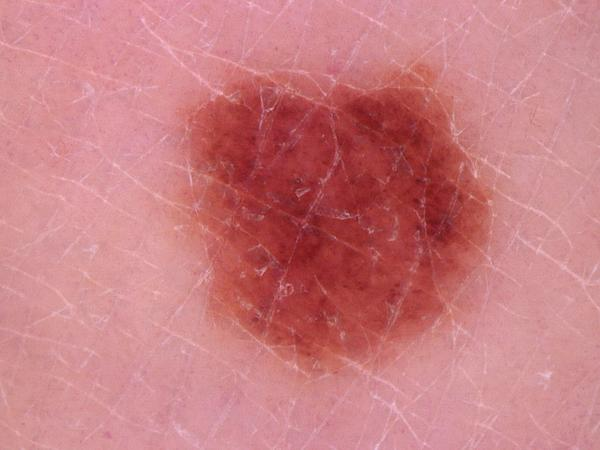
\includegraphics[width=8cm,height=8cm]{derma.jpg}};
% conv1_1,conv1_2,%pool1 

\pic[shift={(0,0,0)}] at (0,0,0) {RightBandedBox={name=cr1,%
        xlabel={{"32",}},zlabel=I,fill=\ConvColor,bandfill=\ConvReluColor,%
        height=40,width={2},depth=40}};

\pic[shift={(2,0,0)}] at (cr1-east) {RightBandedBox={name=invRes1,%
        xlabel={{"16",}},zlabel=I,fill=\InverseResidual,%
        height=40,width={1},depth=40}};

\pic[shift={(2,0,0)}] at (invRes1-east) {RightBandedBox={name=invRes2,%
        xlabel={{"24",}},zlabel=$I/2^{1}$,fill=\InverseResidual,%
        height=35,width={1.5},depth=35}};

\pic[shift={(2,0,0)}] at (invRes2-east) {RightBandedBox={name=invRes3,%
        xlabel={{"24",}},zlabel=$I/2^{1}$,fill=\InverseResidual,%
        height=35,width={1.5},depth=35}};

\pic[shift={(2,0,0)}] at (invRes3-east) {Ball={name=ellipsis0,%
        fill=\ellipsis,opacity=0.6,%
        radius=.2,logo=.}};

\pic[shift={(0.1,0,0)}] at (ellipsis0-east) {Ball={name=ellipsis1,%
        fill=\ellipsis,opacity=0.6,%
        radius=.2,logo=.}};

\pic[shift={(0.1,0,0)}] at (ellipsis1-east) {Ball={name=ellipsis2,%
        fill=\ellipsis,opacity=0.6,%
        radius=.2,logo=.}};

\pic[shift={(1.5,0,0)}] at (ellipsis2-east) {RightBandedBox={name=invRes4,%
        xlabel={{"160",}},zlabel=$I/2^{4}$,fill=\InverseResidual,%
        height=15,width={10},depth=15}};

\pic[shift={(1.5,0,0)}] at (invRes4-east) {RightBandedBox={name=invRes5,%
        xlabel={{"320",}},zlabel=$I/2^{4}$,fill=\InverseResidual,%
        height=15,width={16},depth=15}};

\pic[shift={(1.5,0,0)}] at (invRes5-east) {RightBandedBox={name=cr2,%
        xlabel={{"1280",}},zlabel=$I/2^{4}$,fill=\ConvColor,bandfill=\ConvReluColor,%
        height=15,width={25},depth=15}};

\pic[shift={(3,0,0)}] at (cr2-east) {RightBandedBox={name=fc1,caption=fc+softmax,%
        xlabel={{"1","dummy"}},fill=\FcColor,bandfill=\FcReluColor,%
        height=3,width=3,depth=25}};

%%%%%%%%%%
% softmax
\pic[shift={(0,0,0)}] at (fc1-east) {Box={name=softmax,%
        xlabel={{"","dummy"}},zlabel=K,opacity=0.8,fill=\SoftmaxColor,%
        height=3,width=1.5,depth=25}};

%%%%%%%%%%%%%%%%%%%%%%%%%%%%%%%%%%%%%%%%%%%%%%%%%%%%%%%%%%%%%%%%%%%%%%%%%%%%%%%%%%%%%%%%
%% Draw Dotted Edges 
%%%%%%%%%%%%%%%%%%%%%%%%%%%%%%%%%%%%%%%%%%%%%%%%%%%%%%%%%%%%%%%%%%%%%%%%%%%%%%%%%%%%%%%%
\draw[densely dashed]
    (fc1-west)++(0, 1.5*.2, 1.5*.2) coordinate(a) -- (cr2-nearnortheast)
    (fc1-west)++(0,-1.5*.2, 1.5*.2) coordinate(b) -- (cr2-nearsoutheast)
    (fc1-west)++(0,-1.5*.2,-1.5*.2) coordinate(c) -- (cr2-farsoutheast)
    (fc1-west)++(0, 1.5*.2,-1.5*.2) coordinate(d) -- (cr2-farnortheast)
    
    (a)--(b)--(c)--(d)
    ;
%%%%%%%%%%%%%%%%%%%%%%%%%%%%%%%%%%%%%%%%%%%%%%%%%%%%%%%%%%%%%%%%%%%%%%%%%%%%%%%%%%%%%%%%

%%%%%%%%%%%%%%%%%%%%%%%%%%%%%%%%%%%%%%%%%%%%%%%%%%%%%%%%%%%%%%%%%%%%%%%%%%%%%%%%%%%%%%%%
%% Draw connections
%%%%%%%%%%%%%%%%%%%%%%%%%%%%%%%%%%%%%%%%%%%%%%%%%%%%%%%%%%%%%%%%%%%%%%%%%%%%%%%%%%%%%%%%
\draw [connection]  (cr1-east)    -- node {\midarrow} (invRes1-west);
\draw [connection]  (invRes1-east)    -- node {\midarrow} (invRes2-west);
\draw [connection]  (invRes2-east)    -- node {\midarrow} (invRes3-west);
\draw [connection]  (invRes4-east)    -- node {\midarrow} (invRes5-west);
\draw [connection]  (invRes5-east)    -- node {\midarrow} (cr2-west);
%%%%%%%%%%%%%%%%%%%%%%%%%%%%%%%%%%%%%%%%%%%%%%%%%%%%%%%%%%%%%%%%%%%%%%%%%%%%%%%%%%%%%%%%

\end{tikzpicture}
\end{document}\grid
